\documentclass{article} % Класс печатного документа

\usepackage{hyperref} % Для вставки гиперссылок
\usepackage{listings} % Для вставки кусков кода
\usepackage{graphicx} % Вставка изображений
\usepackage[utf8]{inputenc} % Кодировка исходного текста - utf8
\usepackage[english,russian]{babel} % Поддержка языка - русского с английским
\usepackage{indentfirst} % Отступ в первом абзаце

\title{Отчёт 6\protect\\Скрытые модели Маркова} % Заголовок документа
\author{Свичкарев А.\,В.} % Автор документа
\date{\today} % Текущая дата

\begin{document} % Конец преамбулы, начало текста

\maketitle % Печатает заголовок, список авторов и дату

\section{Задание №1}
Предсказание статусов (buried, exposed) для последовательности\newlineпротеина:

\begin{verbatim}
MYGKIIFVLLLSEIVSISASSTTGVAMHTSTSSSVTKSYISSQTNDTHKRDTYAATPRA
----*******--**------------------------*-------------------
HEVSEISVRTVYPPEEETGERVQLAHHFSEPEITLIIFGVMAGVIGTILLISYGIRRLI
-----***--*----------*----------***********************--**
KKSPSDVKPLPSPDTDVPLSSVEIENPETSDQ
------*-------------------------
\end{verbatim}

\section{Задание №2}
График вероятностей двух состояний аминокислот из заданной последовательности белка: buried (black) и exposed (grey) для каждой позиции марковской цепи:

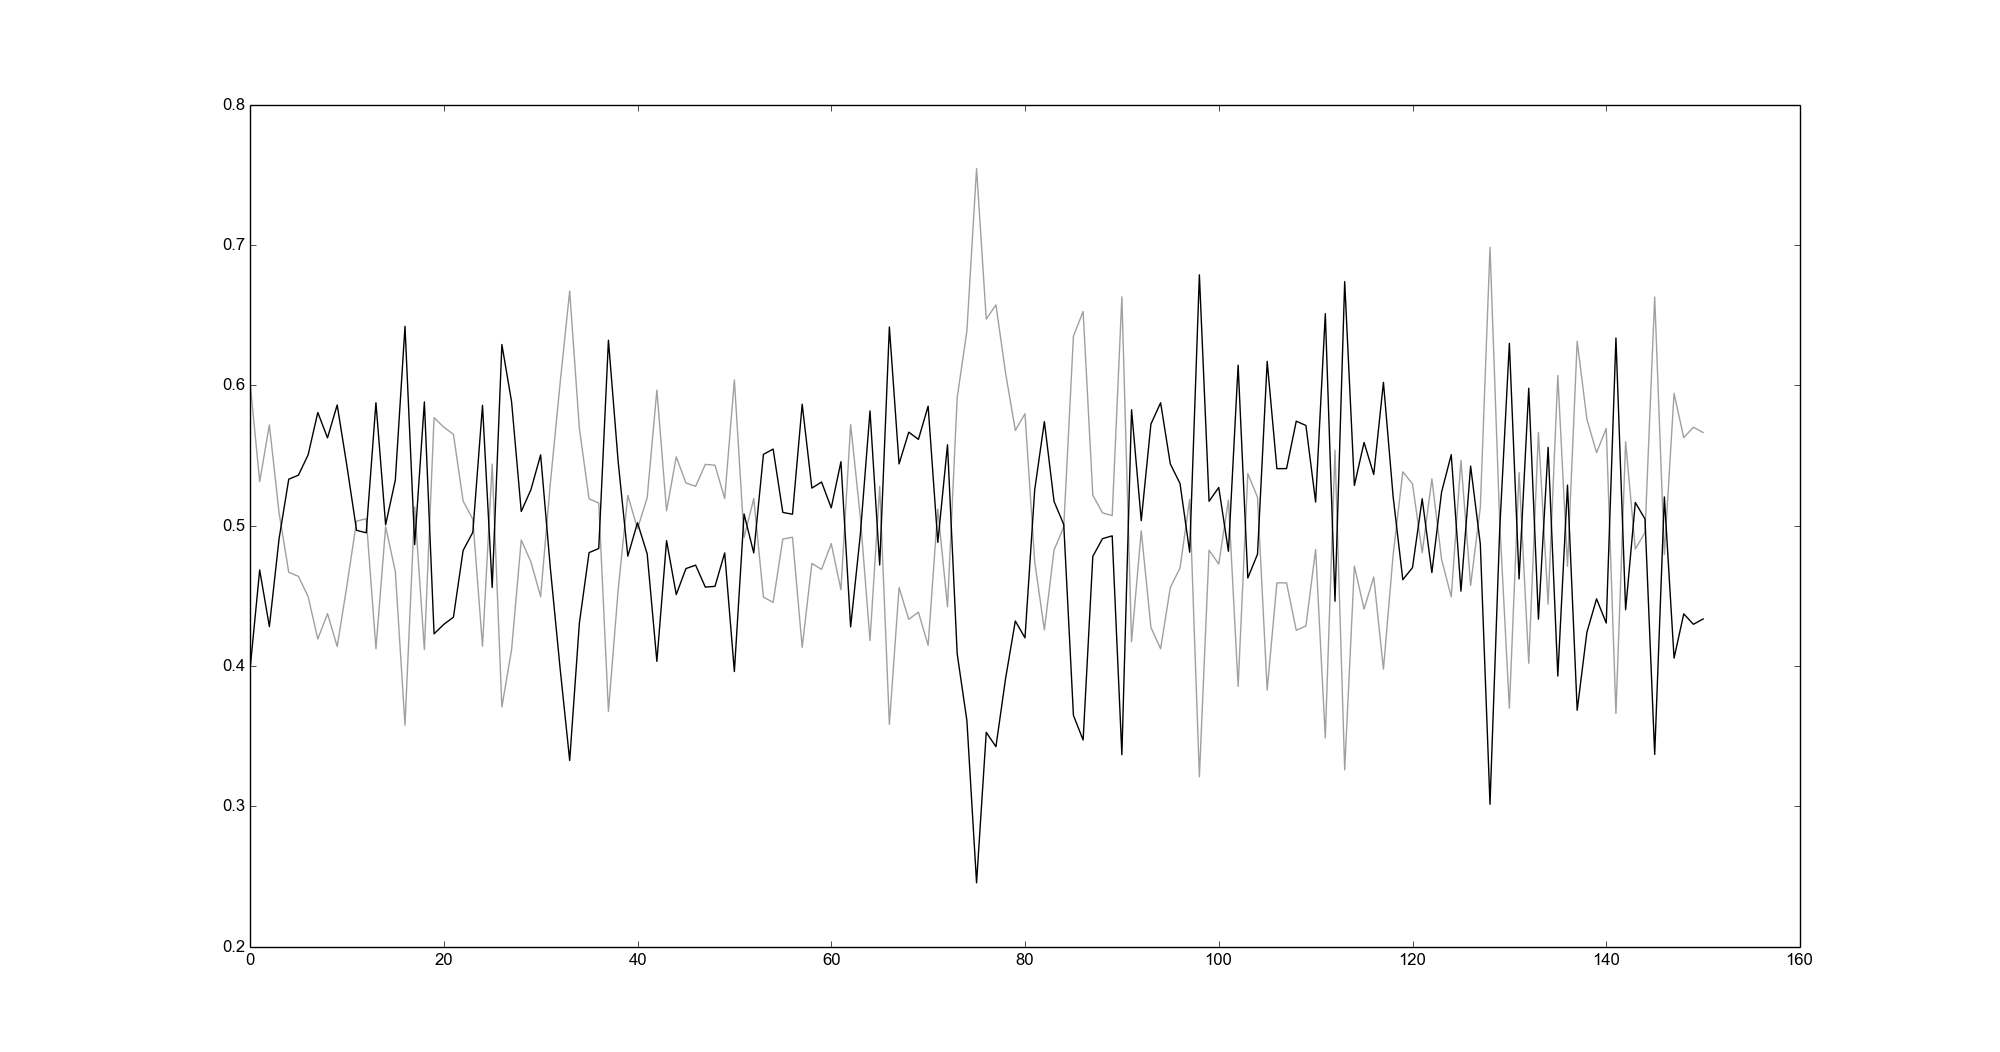
\includegraphics[width=\textwidth]{figure_1}

\section{Пояснение}
За основу был взят и разобран код программы из Приложения:
\begin{itemize}
	\item Был произведён рефакторинг кода в соответствии с \href{https://www.python.org/dev/peps/pep-0008/}{PEP 0008 -- Style Guide for Python Code} рекомендациями.
	\item Были удалены не используемые функции binomialProbability(n, k, p) и getNextGenPop(currentPop, randVar).
	\item Был выделен класс HMM скрытой Марковской модели, который улучшает читабельность кода и инкапсулирует служебные данные. Классу предоставлен интерфейс, который позволяет анализировать новую последовательность с помощью методов класса.
	\item Были доработаны мелкие детали кода. Например, переменная index2 может использоваться без инициализации, если внутренний цикл for не исполнится ни одного раза, что приведёт к ошибке.
\end{itemize}

\section{Исходный код}
\lstinputlisting[language=Python]{../code.py}

\end{document} % Конец документа
